\section{Particles in the heliosphere}
\label{sec:particles_heliosphere}

Our heliosphere is an enormous region in space embedded in the \ac{ISM}, which encompasses all solar system planets and extends far beyond even the Kuiper belt. 
It is filled with a thin plasma consisting of various populations of particles, many of which originate from the Sun itself (\autoref{fig:heliospheric_energy_spectrum}). 
The most abundant population is the solar wind, a steady flow of plasma that is emitted from the Sun radially. 
In the near-Earth space, the slow solar wind reaches typical speeds between \SIrange[range-phrase={\,and\,}]{300}{500}{\kilo\meter\per\second}.
Due to its low pressure, and therefore high plasma $\beta$, it carries the solar magnetic field with it and forms the \ac{IMF}.
As the Sun rotates, the \ac{IMF} carried by the solar wind is shaped like an Archimedian spiral, which is named Parker spiral after Eugene N. \citet{Parker-1958}.

\begin{figure}
    \centering
    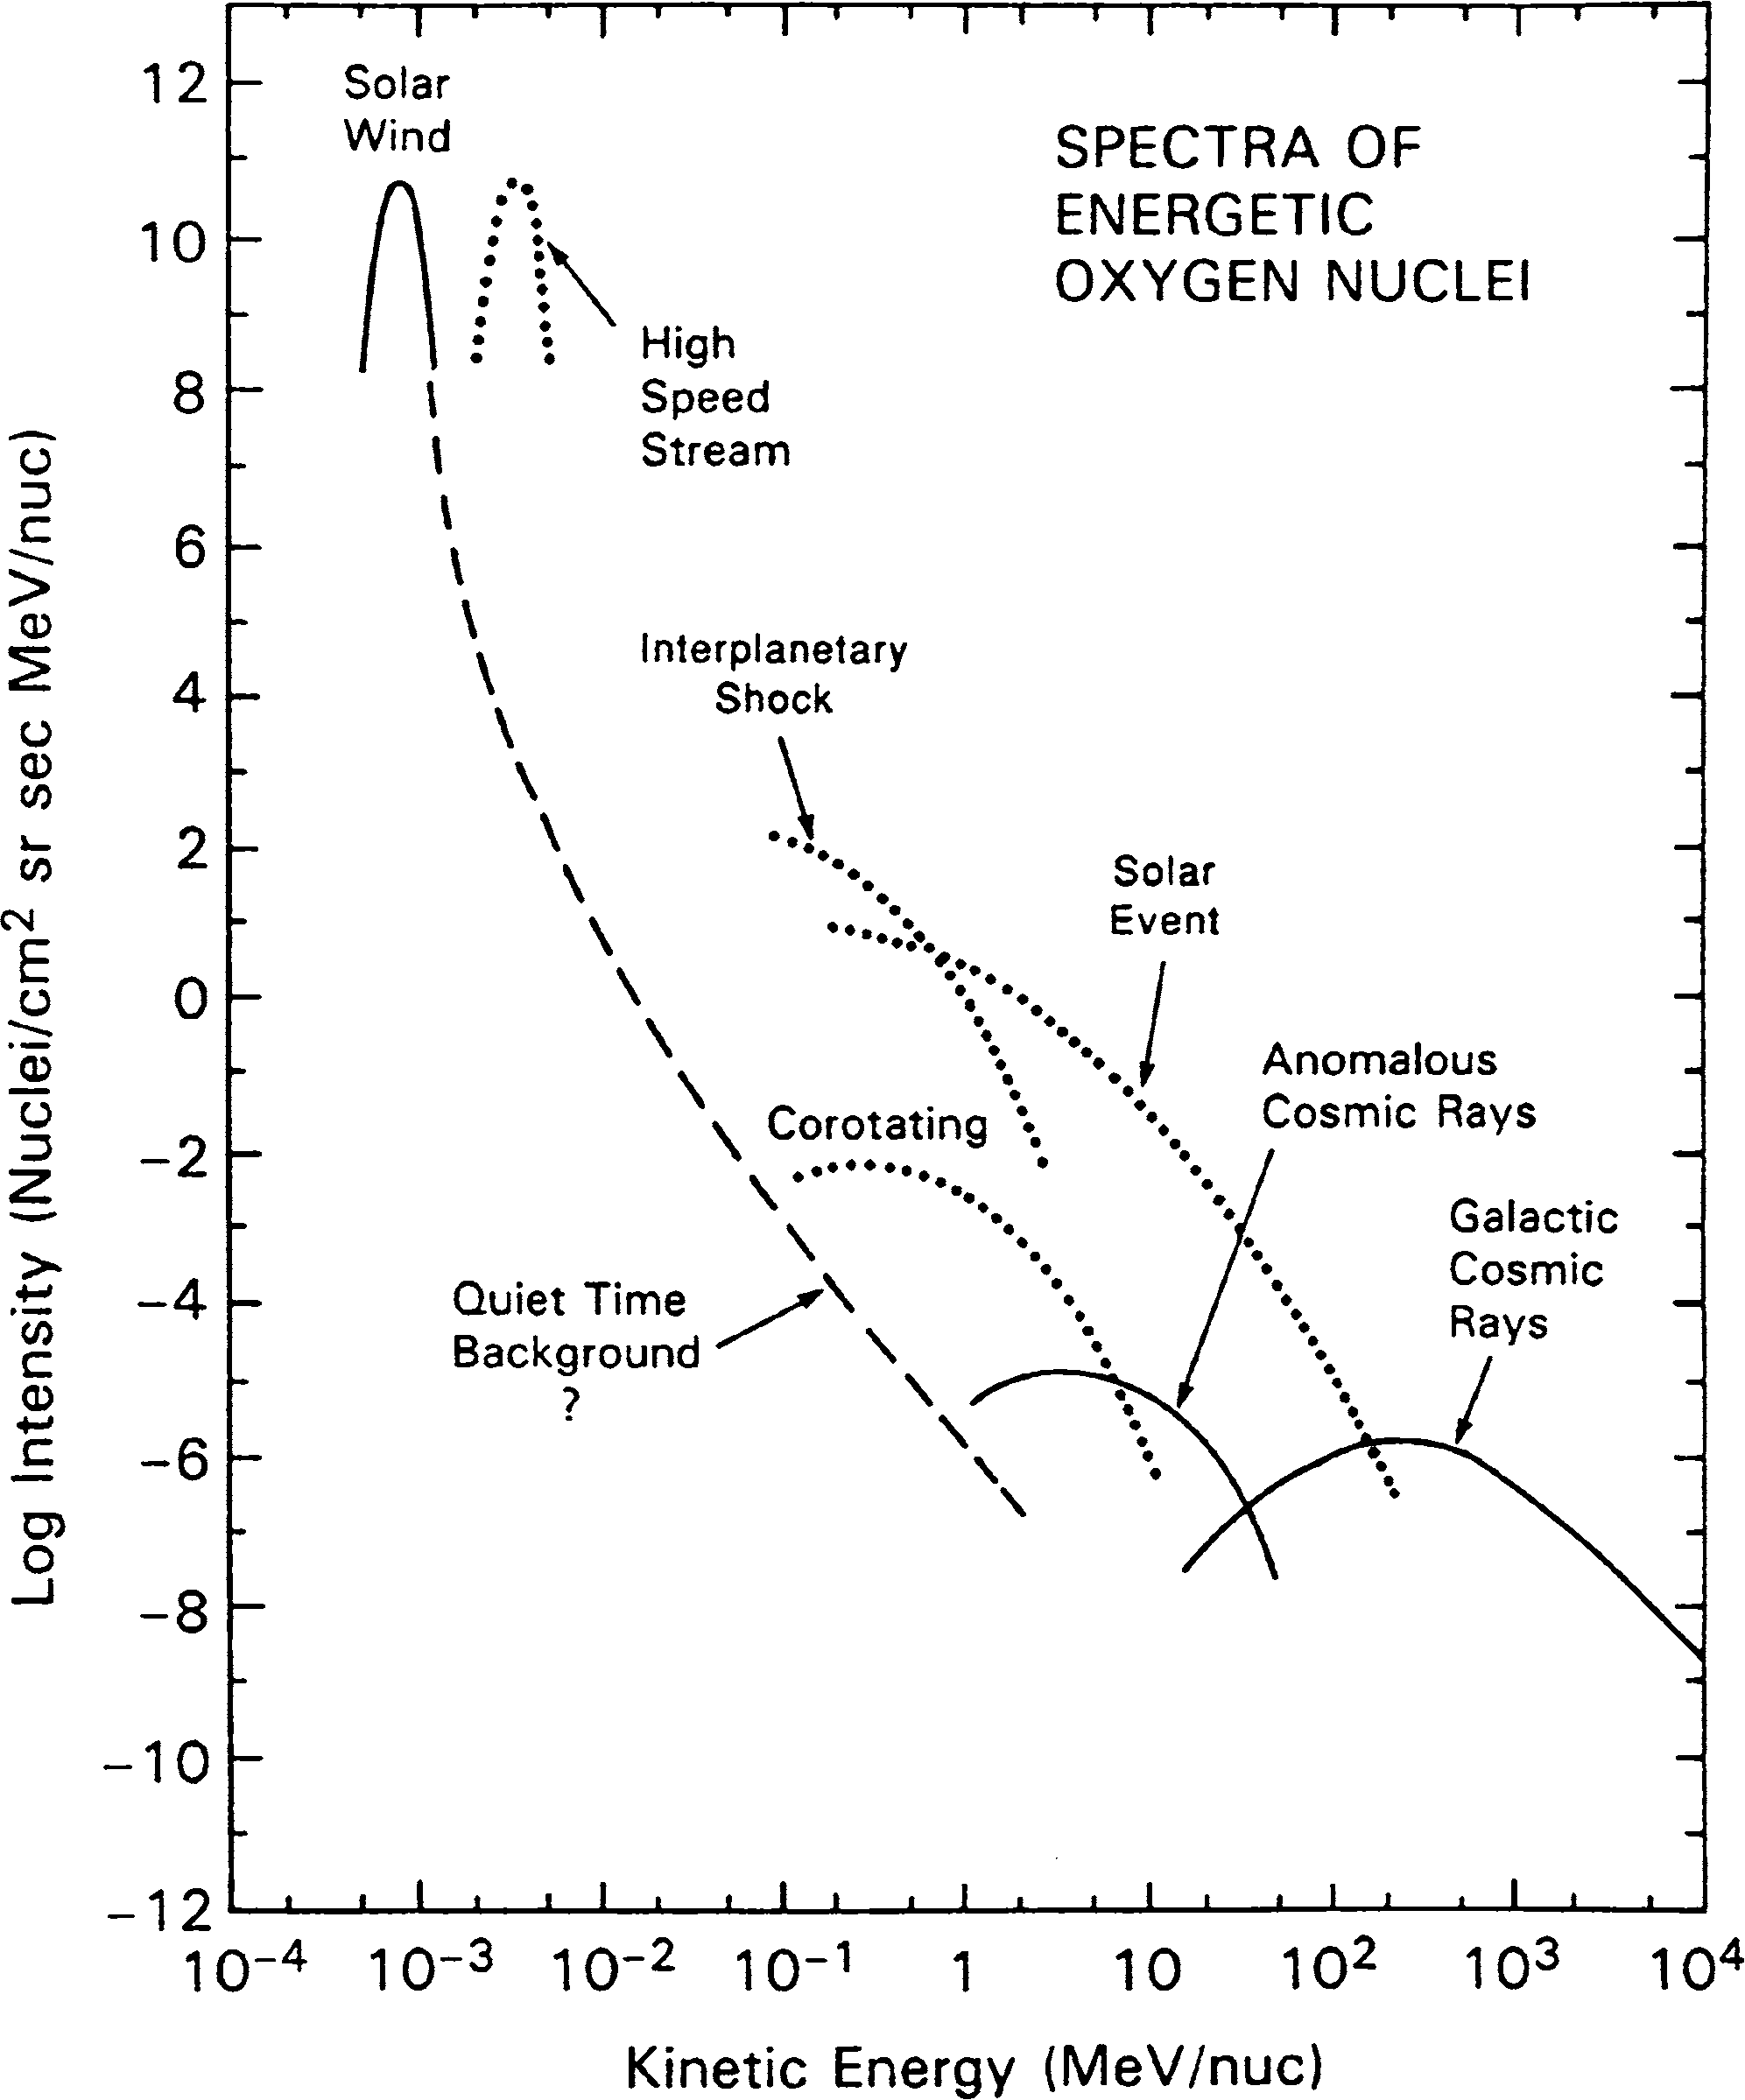
\includegraphics[width=0.6\linewidth]{images/heliospheric_energy_spectrum}
    \caption[Spectra of oxygen ions in the near-Earth interplanetary space]{Typical spectra of oxygen ions in the near-Earth interplanetary space, showing the contributions from different populations. Other particle species show similarly shaped spectra when plotted as a function of energy/nucleon. (adapted from \url{http://helios.gsfc.nasa.gov/ace/gallery.html}, based on \citet{Mewaldt-2001}).}
    \label{fig:heliospheric_energy_spectrum}
\end{figure}

However, our Sun is an active star, and thus, the flow of particles is not simply constant.
Coronal holes forming on the solar surface emit faster solar wind streams with speeds $\gtrsim \SI{600}{\kilo\meter\per\second}$, which interact with the neighboring streams of slower wind by forming a \ac{SIR}. If a coronal hole stays stable for multiple solar rotations, these interaction regions can be observed recurrently, in which case they are called \acp{CIR}.
Furthermore, active regions on the Sun can occasionally produce solar flares, sudden and intense emissions of light often associated with the release of high-energy ($\sim \si{\mega\electronvolt}$) \acp{SEP}.
These are believed to be powered by reconnection of magnetic field lines at the Sun, which leads to the release of energy and acceleration of particles.
They often also coincide with the eruption of plasma from the solar corona in the form of a \ac{CME} at speeds ranging from a few hundreds up to a few thousands of \si{\kilo\meter\per\second}.
Just like the solar wind, \acp{CME} carry a magnetic field with them, often in the form of a flux rope propagating away from the Sun. Due to their high speed, a shock can form in front of the flux rope, followed by a turbulent sheath region.
This shock can also be efficient at accelerating additional particles to higher energies, similar to \acp{SEP} particles accelerated directly at the Sun.

At the high end of the energy spectrum (\autoref{fig:heliospheric_energy_spectrum}) up to \si{\giga\electronvolt} energies, we find \acp{GCR}, particles originating from outside the heliosphere and entering it with a relatively constant and isotropic flux. 
The flux of these high-energy particles within the heliosphere is modulated by various effects: In the long term, the variation of the \ac{IMF} intensity during the 22-year solar cycle causes the average \ac{GCR} flux to be higher during solar minimum than at solar maximum \citep{Fisk-1980}. In addition, there are short-term modulations of \ac{GCR} due to magnetic structures in the solar wind, such as \acp{CME} and \acp{SIR}/\acp{CIR}, so-called Forbush decreases.

% TODO: add citations.

\section{Space Weather events and their detection}
\label{sec:spaceweather}

As defined by the U.S. National Space Weather Program \parencite{OFCM-1995}, the term \textit{space weather} refers to ``conditions on the Sun and in the solar wind, magnetosphere, ionosphere and thermosphere that can influence the performance and reliability of space-borne and ground-based technological systems and endanger human life or health''.
The aforementioned short-term heliospheric events, such as \acp{SEP}, \acp{CME} and \acp{CIR} are all relevant to space weather science, as both the increased radiation exposure due to accelerated energetic particles as well as the magnetic field disturbances, which impact spacecraft or impact the Earth's magnetosphere in a so-called magnetic storm, can have such impacts on technology or human life on Earth, in space, and on other planets.

Thus, the focus in space weather research is to enhance the understanding of these events in order to be able to more accurately predict their occurrence, including the onset time and intensity.
In the past, the development of such models has been mostly based on two kinds of measuremets: Remote-sensing observations of the Sun and its vicinity, such as \ac{EUV} images, magnetograms and white-light coronagraphs, which are available from spacecraft such as \acs{SOHO} and \acs{SDO}, as well as in situ observations at or near Earth, using plasma measurements and magnetometers on spacecraft orbiting Earth (e.g., IMP-8, GOES) or at the $L_1$ Lagrange point (\acs{ACE}, \acs{SOHO}, Wind, \acs{DSCOVR}).
In the last two decades, such observations have been complemented by in situ measurements from deep space heliophysics missions, such as from the two \ac{STEREO} spacecraft orbiting the Sun near \SI{1}{\AU} as well as the recent \ac{PSP} and \ac{SolO} missions, which are starting to provide valuable data from extremely close to the Sun. Additionally these missions facilitate imaging observations from additional vantage points, and these do not only cover the Sun and the corona, but also provide a wide-angle view of interplanetary space using their \acp{HI}, which can be used to directly track \acp{CME} all the way out to Earth.

\section{CMEs, ICMEs and Forbush decreases}
\label{sec:cmes_forbush}

As mentioned in Section \ref{sec:particles_heliosphere}, \acp{CME} are large-scale eruptions of plasma from the Sun that propagate outward into the heliosphere. CMEs occur relatively frequently, on average approximately every 4 days at solar minimum, and 2.5 to 3 times per day at solar maximum \citep{Webb-1994}. The properties of CMEs have a large variability: E.g., their speeds can range between \SIrange[range-phrase={\,and\,}]{20}{2000}{\kilo\meter\per\second}, where the average is at about \SI{400}{\kilo\meter\per\second} and faster CMEs are more likely to occur near solar maximum. The longitudinal extent can also differ, very narrow (\SI{5}{\degree}) and very wide (\SI{120}{\degree}) cases have been observed, with the average being around \SI{50}{\degree} \citep{Cane-2000}.
When the counterparts of CMEs are observed in situ in interplanetary space, they are often referred to as an \ac{ICME}. Common \ac{ICME} signatures include a low proton temperature and density, an enhanced and often smoothly rotating magnetic field (magnetic cloud), bidirectional electron streaming, as well as the modulation of some elemental abundance ratios \citep{Richardson-Cane-1995,Zurbuchen-2006-insitu-signatures,Wimmer-Schweingruber2006}. As it has become clear that the structures observed near the Sun and in interplanetary space are directly linked, especially with the availability of \ac{HI} observations, 

\citet{Forbush-1937} and \citet{Hess-1937} first discovered the influence of \acp{CME} on the \ac{GCR}.

\begin{figure}
    \centering
    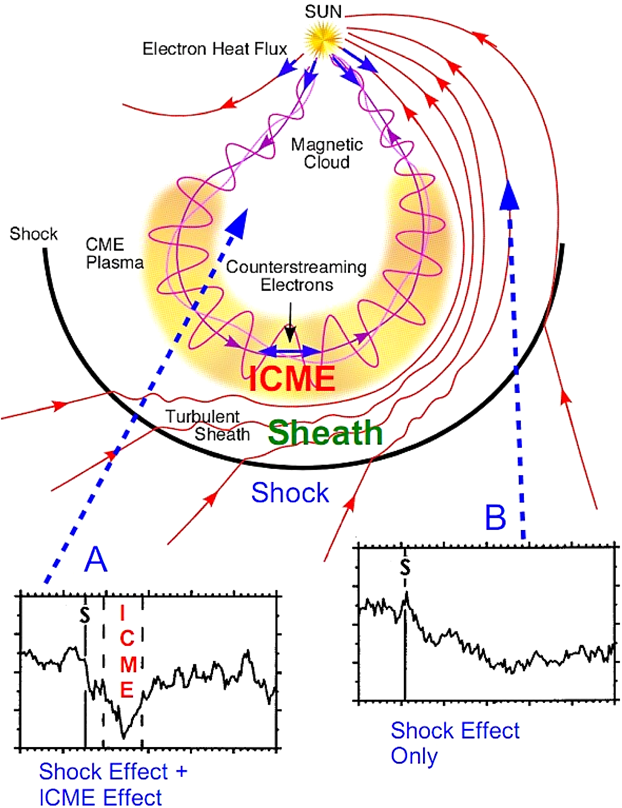
\includegraphics[width=0.6\textwidth]{images/richardson_cane_2011_icme.png}
    \caption{Illustration of an ICME that drives a shock and causes a classical two-step Forbush decrease at location A, where both the shock/sheath and the magnetic cloud pass. At location B, only a single-step Forbush decrease is observed because only the shock is seen here. Source: \citet[Figure 1]{Richardson-Cane-2011}, reprinted by permission from Springer Nature.}
\end{figure}

ground-based neutron monitors or energetic particle detectors


\section{Motivation}



The propagation of 
\acp{FD} have 
